	%-=-=-=-=-=-=-=-=-=-=-=-=-=-=-=-=-=-=-=-=-=-=-=-=
%
%        LOADING DOCUMENT
%
%-=-=-=-=-=-=-=-=-=-=-=-=-=-=-=-=-=-=-=-=-=-=-=-=

\documentclass[newPxFont,pagenumber]{beamer}
\usetheme{sthlm}
%\usecolortheme{sthlmv42}

%-=-=-=-=-=-=-=-=-=-=-=-=-=-=-=-=-=-=-=-=-=-=-=-=
%        LOADING PACKAGES
%-=-=-=-=-=-=-=-=-=-=-=-=-=-=-=-=-=-=-=-=-=-=-=-=
\usepackage[utf8]{inputenc}
\usepackage[frenchb]{babel}
\usepackage[normalem]{ulem}
\usepackage{caption}
\captionsetup{font=scriptsize}
%\usepackage[font=footnotesize]{subcaption}
% in preamble
\usepackage{chronology}
\usepackage{pgf}
\usepackage{tikz}
\usetikzlibrary{arrows,automata}
\usepackage{array,multirow}
\usepackage{nameref}
\makeatletter
\newcommand*{\currentname}{\@currentlabelname}
\makeatother

\graphicspath{ {fig/} }

\usepackage[linesnumbered,ruled,vlined]{algorithm2e}
% add page number
%\usepackage[defaultsans]{cantarell}

\newcommand{\p}{\mathbb{P}}

\setbeamerfont{title}{series=\upshape}
\setbeamertemplate{footline}{\hfill\footnotesize\insertframenumber\hskip3pt\null\vskip3pt}

\newcommand{\argmax}{\mathop{\mathrm{argmax}}\limits}
\renewcommand{\max}{\mathop{\mathrm{max}}\limits}

\renewcommand{\event}[3][e]{%
  \pgfmathsetlength\xstop{(#2-\theyearstart)*\unit}%
  \ifx #1e%
    \draw[fill=black,draw=none,opacity=0.5]%
      (\xstop, 0) circle (.2\unit)%
      node[opacity=1,rotate=45,right=.2\unit] {#3};%
  \else%
    \pgfmathsetlength\xstart{(#1-\theyearstart)*\unit}%
    \draw[fill=black,draw=none,opacity=0.5,rounded corners=.1\unit]%
      (\xstart,-.1\unit) rectangle%
      node[opacity=1,rotate=45,right=.2\unit] {#3} (\xstop,.1\unit);%
  \fi}%

\addto\captionsfrench{%
\renewcommand{\figurename}{\scriptsize {\scshape Figure}}
\renewcommand{\tablename}{\scriptsize {\scshape Table}}
}

%-=-=-=-=-=-=-=-=-=-=-=-=-=-=-=-=-=-=-=-=-=-=-=-=
%        BEAMER OPTIONS
%-=-=-=-=-=-=-=-=-=-=-=-=-=-=-=-=-=-=-=-=-=-=-=-=

%\setbeameroption{show notes}

%-=-=-=-=-=-=-=-=-=-=-=-=-=-=-=-=-=-=-=-=-=-=-=-=
%
%	PRESENTATION INFORMATION
%
%-=-=-=-=-=-=-=-=-=-=-=-=-=-=-=-=-=-=-=-=-=-=-=-=

\title{\vspace{0.4cm}\normalsize Analyse sémantique d’un corpus exhaustif de décisions jurisprudentielles pour l'élaboration d’un modèle prédictif du risque judiciaire     }
\subtitle{\scriptsize Comité de suivi individuel -- \textit{12 juillet 2017}}
%\date{\small{\jobname}}
\date{\scriptsize Début de thèse: 15 Décembre 2015}
\author{\normalsize Gildas Tagny Ngompé}
\institute{\scriptsize \textbf{Direction de thèse:} \begin{itemize}
\item Jacky Montmain (École des mines d'Alès, LGI2P)
\item Stéphane Mussard (Université de Nîmes, CHROME)
\end{itemize}
\textbf{Encadrement de proximité:} \begin{itemize}
\item Sébastien Harispe (Ecole des Mines d'Alès, LGI2P)
\item Guillaume Zambrano (Université de Nîmes, CHROME)
\end{itemize}}

\hypersetup{
pdfauthor = {\author{}: tagnyngompe@gmail.com},
pdfsubject = {},
pdfkeywords = {},
pdfmoddate= {D:\pdfdate},
pdfcreator = {}
}

\begin{document}
\nocite{}
%-=-=-=-=-=-=-=-=-=-=-=-=-=-=-=-=-=-=-=-=-=-=-=-=
%
%	TITLE PAGE
%
%-=-=-=-=-=-=-=-=-=-=-=-=-=-=-=-=-=-=-=-=-=-=-=-=
\begin{frame}[plain]
	\titlepage
\end{frame}
%}
%-=-=-=-=-=-=-=-=-=-=-=-=-=-=-=-=-=-=-=-=-=-=-=-=
%
%	TABLE OF CONTENTS: Plan
%
%-=-=-=-=-=-=-=-=-=-=-=-=-=-=-=-=-=-=-=-=-=-=-=-=
\section*{Plan}
\begin{frame}[c]{\currentname}
\tableofcontents[hideallsubsections]
\end{frame}

\section{Motivations et objectifs}

\begin{frame}[c]{Les juristes analysent les décisions afin d'anticiper}
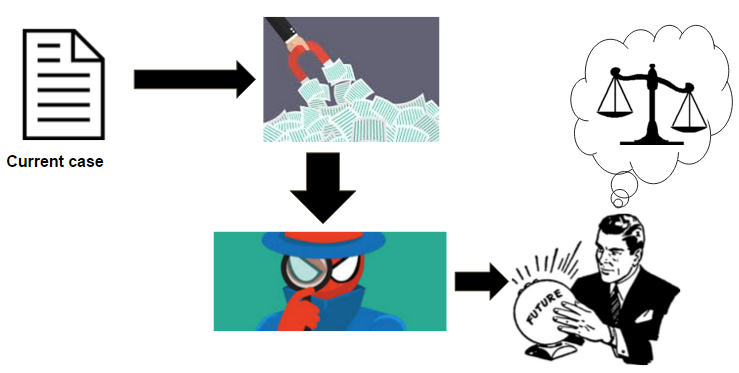
\includegraphics[width=\textwidth]{lawyerwork.png}
\end{frame}

\begin{frame}[c]{Défis: grand volume de décisions}
\textbf{Plus de 4 millions de décisions prononcées / an}
\begin{table}[!htb]
{
\footnotesize
\begin{center}
\begin{tabular}{|p{2cm}|c|c|c|c|c|}
\hline
 & \textbf{2010} & \textbf{2011} & \textbf{2012} & \textbf{2013} & \textbf{2014} \\
 \hline
 \textbf{Justice civile} & 2 673 131  & 2 654 179 & 2 647 813 & 2 761 554  & 2 618 374 \\
 \hline
\textbf{Justice pénale} & 1 173 242 & 1 180 586 & 1 251 979 & 1 303 469 & 1 203 339 \\
 \hline
 \textbf{Justice administrative} & 224 787 & 225 608 & 228 680 & 221 882 & 230 477 \\
 \hline
\end{tabular}
\textit{\tiny{Source: \url{http://www.justice.gouv.fr/budget-et-statistiques-10054/chiffres-cles-de-la-justice-10303/}}}  
\end{center}
}
\caption{Nombre de décisions prononcées en France par an}\label{decisionstats}
\end{table}
\end{frame}

\begin{frame}[t]{Défis: Recherches et analyses sémantiques difficiles}

Moteurs de recherche juridique à mots-clés 

Pas d'analyse synthétique des décisions 

%\begin{figure}
\fbox{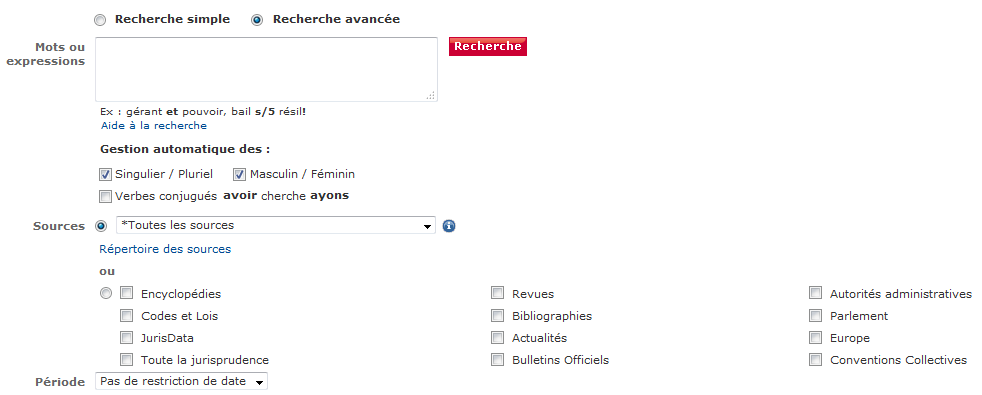
\includegraphics[width=0.9\paperwidth]{jurica.png}}

\textit{\tiny{Source: \url{LexisNexis.com}}} 
%\caption{Formulaire de recherche}
%\end{figure}
\end{frame}


\begin{frame}{Défis: Documents non-structurés}
\scriptsize
\begin{columns}
\begin{column}{.50\linewidth}
ARRÊT N°

R.G: 11/03924

...

{COUR D'APPEL} DE {NÎMES}

{CHAMBRE CIVILE}

{1ère Chambre A}

ARRÊT DU {20 MARS 2012}

APPELANTE:

{Madame Michéle A.} ...

assistée de la {SELARL VAJOU}, ...

INTIMES:

{Monsieur Martial B} ...

assisté de la {SCP MARION GUIZARD PATRICIA SERVAIS}, ...

COMPOSITION DE LA COUR LORS DU DÉLIBÉRÉ:

{M. Dominique BRUZY, Président}

{M. Serge BERTHET, Conseiller}

...
\end{column}
\begin{column}{.50\linewidth}
FAITS, PROCEDURE, ...

Madame Michèle A. demande:

...

- de condamner Madame JONES-B. à lui payer la somme de {2.500 euros} au titre de l'{article 700 du Code de Procédure Civile}, 

\vspace{0.4cm}

PAR CES MOTIFS, LA COUR:

...

Vu l'{article 809 du Code de Procédure Civile},

...

{Déboute Madame A. de sa demande de provision sur dommages-intérêts.}

...

Vu l'{article 700 du Code de Procédure Civile},

Condamne Madame JONES-B. à verser à Madame A. la somme de {2.500 euros}.
\end{column}
\end{columns}
\end{frame}

\begin{frame}{Notre projet: Automatiser la structuration et l'analyse}
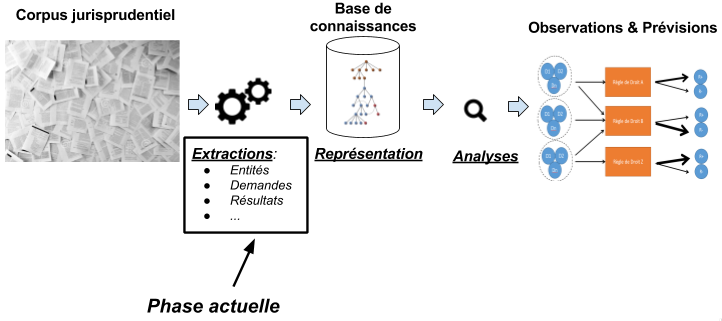
\includegraphics[width=\textwidth]{pipeline-cassandra2.png}

Elaboration et mise en oeuvre de techniques de :
\begin{itemize}
\item Traitement du langage naturel 

\item Représentation des connaissances
 
\item Recherche d'information
\end{itemize}

\end{frame}


%%-=-=-=-=-=-=-=-=-=-=-=-=-=-=-=-=-=-=-=-=-=-=-=-=
%%
%%	Questions
%%
%%-=-=-=-=-=-=-=-=-=-=-=-=-=-=-=-=-=-=-=-=-=-=-=-=
\section{Détection de sections et d'entités}


\begin{frame}{Sectionner les décisions pour organiser l'extraction}
\scriptsize
\begin{columns}
\begin{column}{.45\linewidth}
\fbox{\begin{minipage}{\textwidth}ARRÊT N°

R.G: \textcolor{red}{11/03924}

\textcolor{red}{COUR D'APPEL} DE \textcolor{red}{NÎMES}

\textcolor{red}{CHAMBRE CIVILE}

\textcolor{red}{1ère Chambre A}

ARRÊT DU \textcolor{red}{20 MARS 2012}

APPELANTE:

\textcolor{red}{Madame Michéle A.} ...

assistée de la \textcolor{red}{SELARL VAJOU}, ...

INTIMES:

\textcolor{red}{Monsieur Martial B} ...

assisté de la \textcolor{red}{SCP MARION GUIZARD PATRICIA SERVAIS}, ...

COMPOSITION DE LA COUR LORS DU DÉLIBÉRÉ:

\textcolor{red}{M. Dominique BRUZY, Président}

\textcolor{red}{M. Serge BERTHET, Conseiller}

...
\end{minipage}}
\vspace{0.1cm}

{\normalsize \textbf{Entêtes}: méta-données}
\end{column}
\begin{column}{.55\linewidth}
\fbox{\begin{minipage}{\textwidth}FAITS, PROCEDURE, ...

Madame Michèle A. demande:

...

- de condamner Madame JONES-B. à lui payer la somme de \textcolor{red}{2.500 euros} au titre de l'\textcolor{red}{article 700 du Code de Procédure Civile}, 
\end{minipage}}
\vspace{0.1cm}

{\normalsize \textbf{Corps}: demandes, arguments et normes }

\vspace{0.4cm}

\fbox{\begin{minipage}{\textwidth}PAR CES MOTIFS, LA COUR:

...

Vu l'\textcolor{red}{article 809 du Code de Procédure Civile},

...

\textcolor{red}{Déboute Madame A. de sa demande de provision sur dommages-intérêts.}

...

Vu l'\textcolor{red}{article 700 du Code de Procédure Civile},

Condamne Madame JONES-B. à verser à Madame A. la somme de \textcolor{red}{2.500 euros}.
\end{minipage}}
\vspace{0.1cm}

{\normalsize \textbf{Dispositif}: résultats et normes}

\end{column}
\end{columns}
\end{frame}

\begin{frame}{Entités et sections à détecter}

\scriptsize
\begin{table}[!htb]
\centering
%\scriptsize
\begin{tabular}[c]{|l|c|p{0.6\textwidth}|}
\hline
\textbf{Entités} & \textbf{Labels} & \textbf{Exemples}\\\hline
\multicolumn{3}{|c|}{\textbf{Section entête (E)}} \\
\hline
Numéro R.G. & \textbf{RG} & "10/02324", "60/JAF/09" \\ \hline
Ville & \textbf{VL}& "NÎMES", "Agen", "Toulouse" \\ \hline
Type de juridiction & \textbf{JR} & "COUR D'APPEL" \\ \hline
Formation & \textbf{FM} & "1re chambre", "Chambre économique" \\ \hline
Date & \textbf{DT} & "01 MARS 2012", "15/04/2014"\\ \hline
Partie appelante & \textbf{AP} & "SARL K.", "Syndicat ...", "Mme X ..."\\ \hline
Partie intimée & \textbf{IM} & - // - \\ \hline
Partie intervenante & \textbf{IV} & - // - \\ \hline
Avocat & \textbf{AV} & "Me Dominique A., avocat au barreau de Papeete"\\ \hline
Juge & \textbf{JG} & "Monsieur André R.", "Mme BOUSQUEL" \\ \hline
fonction du juge & \textbf{FT} & "Conseiller", "Président"\\ \hline
\multicolumn{3}{|c|}{\textbf{Corps (T) et dispositif (D)}} \\ \hline

Norme & \textbf{NO} & "l' article 700 NCPC", "articles 901 et 903"  \\ \hline
\hline
Élément à éviter & \textbf{O} & \textit{tout élément ne faisant partie d'aucune entité ciblée} \\ \hline
\end{tabular} 

\caption{Entités et leurs labels par section.}\label{relevantinfo}
\end{table}
\end{frame}

\begin{frame}{Architecture proposée}
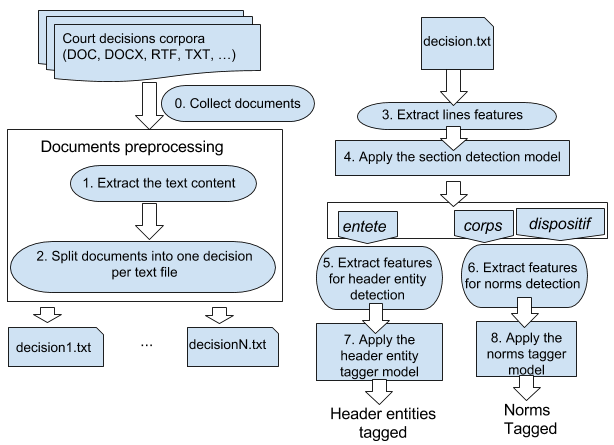
\includegraphics [width=\textwidth]{archAppli.png}
\end{frame}


\begin{frame}{Approches probabilistes d'étiquetage de séquence}
Modèles probabilistes à états et observations

\scriptsize
\begin{table}[]%width=\linewidth
	%\begin{tabular}[]{p{0.40\linewidth}|p{0.55\linewidth}}
	\begin{tabular}[]{c|c}
		\toprule
{\textbf{HMM}} & {\textbf{CRF}} \\
%		\midrule
%		\textbf{Generative} models 	& \multicolumn{2}{c}{"\textbf{Discriminative}" or "\textbf{Conditional}" models } \\[0.25em]
%\midrule		
%"\textbf{generate}" input	& {"\textbf{condition}" on input }\\%[0.25em]
\midrule
{un seul descripteur  par observation}	& {plusieurs descripteurs complexes par observation}\\%[0.25em]
\midrule	
		\begin{tikzpicture}[->,>=stealth',shorten >=1pt,auto,node distance=1.3cm,
                    semithick]
  \node[state] (S1)                    {$s_{t-1}$};
  \node[state]         (S2) [right of=S1] 	  {$s_{t}$};
  \node[state]         (O) [below of=S2] {$o_{t}$};
  \path (S1) edge              node {} (S2)
        (S2) edge              node {} (O);
\end{tikzpicture}
				& 

\begin{tikzpicture}[auto,>=stealth',shorten >=1pt,auto,node distance=1.3cm,
                    semithick]
  \node[state] (S1)                    {$s_{t-1}$};
  \node[state]         (S2) [right of=S1] 	  {$s_{t}$};
  \node[state]         (O) [below of=S2] {$o_{t}$};
  \path (S1) edge              node {} (S2)
        (S2) edge              node {} (O);
\end{tikzpicture}					
					\\%[0.25em]
\midrule
$P_\lambda(S,O) = \prod\limits_{t=1}^{T} P(s_t \vert s_{t-1}) * P(o_t \vert s_{t})$  & $P_\lambda(S|O) = \frac{1}{Z(O)}exp\left( \sum\limits_{t=1}^{T}\sum\limits_{k} \lambda_k f_k(s_{t-1},s_t, o_t) \right) $ \\
% & & & \\
\tiny \cite{Seymore1999hmm} & \tiny \cite{peng2006crf} \\ 
		\bottomrule
	\end{tabular}
\end{table}

\normalsize

Objectif: Trouver la séquence la plus probable d'étiquetage pour l'ensemble du texte

\textbf{Entrainement sur des séquences préalablement étiquetées}
\end{frame}

\begin{frame}[c]{Premiers résultats \cite{tagny2017sectNerhmmcrf}}
\begin{table}[!htb]
\scriptsize

\centering
\begin{tabular}{|c|c|c|c|c|c|c|c|c|c|}
\hline
 & \multicolumn{3}{c|}{HMM}  & \multicolumn{3}{c|}{CRF-}  & \multicolumn{3}{c|}{CRF+} \\
\hline
\textit{labels} & P & R & F1 & P & R & F1 & P & R & F1 \\
\hline
 \multicolumn{10}{|c|}{\textit{\textit{Section Entête (E)}}} \\
\hline
 AP & 35.3 &  14.1 & 20.1  & 64.9 & 48.8 & 55.6 & 92.0 & 86.7 & 89.3 \\
\hline
 AV & 83.8 &  98.3 & 90.5  & 96.4 & 97.5 & 96.9 & 97.6 & 98.1 & 97.9 \\
 \hline
 DT & 70.9 & 72.6 & 71.7  & 94.4 & 86.8 & 90.4 & 98.8 & 97.7 & 98.2 \\
 \hline
FM & 87.6 &  93.7 & 90.5  & 98.8 & 98.4 & 98.6 & 98.9 & 99.3 & 99.1 \\
 \hline
FT &  88.8 & 59.8 & 71.3  & 94.2 & 92.3 & 93.3 & 97.1 & 95.5 & 96.3 \\
 \hline
IM  & 53.1 & 57.4 & 55.1  & 67.2 & 64.6 & 65.8 &  89.3 & 88.1 & 88.7  \\
 \hline
 \textcolor{red}{IV} & - & 2.2 & - & 25.9 & 26.5 & 26.2 & 67.3 & 41.4 & \textcolor{red}{46.4} \\
 \hline
JG  & 68.0 & 85.7 & 75.7  & 96.2 & 95.7 & 96.0 & 98.1 & 97.7 & 97.9 \\
 \hline
JR  & 75.8 & 99.5 & 86.0  & 98.6 & 99.4 & 99.0 & 99.3 & 99.4 & 99.4 \\
 \hline
RG  &  - & 0  & - & 83.7 & 46.1 & 59.4 & 98.6 & 97.4 & 98.0 \\
\hline
VL & 93.1 & 27.9 & 42.6  & 98.2 & 98.4 & 98.3 & 99.0 & 99.0 & 99.0 \\
\hline
 \multicolumn{10}{|c|}{\textit{\textit{Sections inférieures (T \& D )}}} \\
 \hline
NO & 92.9 & 90.9 & 91.9 & 96.0 & 93.8 & 94.9 & 97.9 & 96.5 & 97.2\\
\hline
\end{tabular}
\caption{Précision (P), rappel (R), F1-mesure (F1) au niveau des mots ($\%$).}\label{prf-entity}
\end{table}
\end{frame}

\begin{frame}{Premiers travaux \cite{tagny2017sectNerhmmcrf}}
\begin{itemize}
\item Utilité de la prise en compte des particularités des textes
\begin{itemize}
\item forme : le mot est-il en majuscule, lemmes, longueur de la ligne, ...
\item contexte : mots voisins, position par rapport à un mot-clé, ...
\end{itemize}
\item Certaines entités restent difficiles à détecter
\end{itemize}

\vspace{1.5cm}

\textbf{\Large \textit{Comment améliorer les résultats ?}}

Définir plus de caractéristiques:

\begin{itemize}
\item 14 pour les sections
\item 35 pour les entêtes
\item 28 pour les normes
\end{itemize}
\end{frame}
%\begin{table}[!htb]
%\scriptsize
%\centering
%\begin{tabular}{|c|c|c|c|c|c|c|c|c|c|}
%\hline
% & \multicolumn{3}{c|}{HMM} & \multicolumn{3}{c|}{CRF-} & \multicolumn{3}{c|}{CRF+} \\
%\hline
% & P & R & F1  & P & R & F1 & P & R & F1 \\
%\hline
%Entête & 84.2 & 91.8 & 87.8  & 93.8 & 85.4 & 89.3 & 99.3 & 99.6 & 99.5 \\
%\hline
%Corps & 88.4 & 63.9 & 74.1  & 86.3 & 98.2 & 91.8 & 99.8 & 99.5 & 99.7\\
%\hline
%Dispositif & 15.4 & 47.0 & 23.0  & 100.0 & 8.5 & 15.6 & 98.0 & 100.0 & 98.9 \\
%\hline
%\textit{Moyenne} & 62.7 & 67.6 & 67.6  & 93.3 & 64.0 & 64.0 & 99.7 & 99.8 & 99.8  \\
%\hline
%\end{tabular}
%\caption{Précision (P), rappel (R), F1-mesure (F1) au niveau des lignes ($\%$).}
%\label{prf-zoning}
%\end{table}

\begin{frame}{Résultats avec plus de caractéristiques}
\begin{table}
\scriptsize
\begin{tabular}{|l|ccc|}
\hline
         & Precision &  Recall  & F1 \\\hline
I-corps &   99.57\% &  99.69\% &  99.63 \\
I-dispositif &   98.63\% &  97.59\% &  98.11 \\
I-entete &   99.51\% &  99.55\% &  99.53 \\\hline
Overall &   99.48\% &  99.48\% &  99.48 \\\hline
 \noalign{\smallskip}\hline\noalign{\smallskip}
I-appelant &   84.34\% &  76.27\% &  80.10 \\
I-avocat &   98.02\% &  98.15\% &  98.09 \\
I-date  &   98.00\% &  96.60\% &  97.30 \\
I-fonction &   95.23\% &  95.13\% &  95.18 \\
I-formation &   98.80\% &  99.45\% &  99.12 \\
I-intervenant &   83.38\% &  68.26\% &  \textcolor{red}{75.07} \\
I-intime &   82.54\% &  83.33\% &  82.93 \\
I-juge  &   97.55\% &  97.23\% &  97.39 \\
I-juridiction &   98.91\% &  99.69\% &  99.30 \\
I-rg    &   97.81\% &  97.44\% &  97.62 \\
I-ville &   98.94\% &  99.15\% &  99.04 \\\hline
Overall &   95.13\% &  94.51\% &  94.82 \\\hline
 \noalign{\smallskip}\hline\noalign{\smallskip}
I-norme &   97.14\% &  96.09\% &  96.62 \\\hline
\end{tabular}
\caption{Résultats du CRF avec l'ajout de caractéristiques.}
\end{table}
\end{frame}


\begin{frame}{Sélection des caractéristiques}
\begin{table}[!h]
\tiny
\begin{tabular}{l|c|ccc}
\hline\noalign{\smallskip}
Detection Task & Tagger & {Token-level F1} & {Entity-level F1}& Features subset \\ \hline
%\noalign{\smallskip}\svhline\noalign{\smallskip}
\multirow{7}{*}{Sections} 		& \multirow{4}{*}{CRF} & 99.31 & 90.48 & BDS  \\
  				&  & \textbf{99.55} & 85.76 & \textbf{SFFS} \\
                &  & 99.46 & 90.03 & ALL \\
                &  & 91.75 & 60.26 & token \\  \cline{2-5}
                 & \multirow{3}{*}{HMM} & \textbf{90.99} & 3.89 & \textbf{absLength} \\ 
 & & 86.97 & 3.65 & relLength \\   
  &  & 37.59 & 18.81 & token \\ \hline
\multirow{7}{*}{Header entities}	& \multirow{4}{*}{CRF} & 92.69 & 90.47 & BDS  \\
				&  & \textbf{93.00} & 90.76 & \textbf{SFFS}  \\ 
                &  & 92.74 & 90.81 & ALL \\
                &  & 82.73 & 72.17 & token \\ \cline{2-5}
                  &  \multirow{3}{*}{HMM}  & \textbf{78.61} & \textbf{56.93} &  \textbf{token} \\ 
  &    & 68.04 & 32.96 &  lemma\_W0 \\ 
  &    & 38.54 & 7.95 &  POS \\ \hline
\multirow{6}{*}{Norms} 			& \multirow{4}{*}{CRF} & \textbf{96.31} & 90.80 & \textbf{BDS} \\ 
				&  & 95.57 & 89.29 & SFFS \\ 
                &  & 95.87 & 90.76 & ALL \\
                &  & 94.26 & 85.72 & token \\ \cline{2-5}
                 &  \multirow{2}{*}{HMM} & \textbf{91.66} & \textbf{74.9} &  \textbf{token} \\ 
  &   & 91.54 & 69.35 &  lemma\_W0 \\ 
%  \noalign{\smallskip}\svhline\noalign{\smallskip}
%  & & token-level & entity-level & \\ \hline
%\noalign{\smallskip}\hline\noalign{\smallskip}
\end{tabular}
\caption{Impact de la réduction des caractéristiques}
\end{table}

%Réduit de \textbf{moitié} le nombre de caractéristiques

%Améliore légèrement les résultats

BDS et SFFS \textcolor{red}{très lents (plus de 10 h lors de nos tests)}
\end{frame}

%\begin{frame}{Sélection des caractéristiques}
%\tiny
%\begin{tabular}{l|c|ccc}
%\toprule
%Detection Task & Tagger & {Token-level F1$^a$} & {Entity-level F1$^a$}& Features subset \\ 
%\midrule
%\multirow{7}{*}{Sections} 		& \multirow{4}{*}{CRF} & 99.31 & 90.48 & BDS$^{b1}$  \\
%  				&  & \textbf{99.55} & 85.76 & \textbf{SFFS}$^{b2}$ \\
%                &  & 99.46 & 90.03 & ALL \\
%                &  & 91.75 & 60.26 & token \\  \cline{2-5}
%                 & \multirow{3}{*}{HMM} & \textbf{90.99} & 3.89 & \textbf{absLength} \\ 
% & & 86.97 & 3.65 & relLength \\   
%  &  & 37.59 & 18.81 & token \\ \hline
%\multirow{7}{*}{Header entities}	& \multirow{4}{*}{CRF} & 92.69 & 90.47 & BDS$^{c1}$  \\
%				&  & \textbf{93.00} & 90.76 & \textbf{SFFS}$^{c2}$  \\ 
%                &  & 92.74 & 90.81 & ALL \\
%                &  & 82.73 & 72.17 & token \\ \cline{2-5}
%                  &  \multirow{3}{*}{HMM}  & \textbf{78.61} & \textbf{56.93} &  \textbf{token} \\ 
%  &    & 68.04 & 32.96 &  lemma\_W0 \\ 
%  &    & 38.54 & 7.95 &  POS \\ \hline
%\multirow{6}{*}{Norms} 			& \multirow{4}{*}{CRF} & \textbf{96.31} & 90.80 & \textbf{BDS}$^{d1}$ \\ 
%				&  & 95.57 & 89.29 & SFFS$^{d2}$ \\ 
%                &  & 95.87 & 90.76 & ALL \\
%                &  & 94.26 & 85.72 & token \\ \cline{2-5}
%                 &  \multirow{2}{*}{HMM} & \textbf{91.66} & \textbf{74.9} &  \textbf{token} \\ 
%  &   & 91.54 & 69.35 &  lemma\_W0 \\ 
%%  \noalign{\smallskip}\svhline\noalign{\smallskip}
%%  & & token-level & entity-level & \\ \hline
%\bottomrule
%\end{tabular}
%\end{frame}
%
%\begin{frame}{Sélection de la représentation de segment}
%\tiny
%\begin{tabular}{p{0.17\textwidth}|c|cccp{0.18\textwidth}}
%\toprule
%Detection Task & Tagger\hspace{0.1cm} & {Token-level F1$^a$}\hspace{0.1cm} & {Entity-level F1$^a$}\hspace{0.1cm} & training time$^b$\hspace{0.1cm} & Representation \\ 
%\midrule
%\multirow{8}{*}{Sections}  & \multirow{4}{*}{CRF} & 91.75 & 60.26 &  4.685  & IO \\
%&  & 88.95 & 42.63  & 11.877 & IEO2 \\
%&  & 87.09 & 41.45 & 12.256 & BIO2 \\
% &  & 86.00 & 48.97  & 35.981 & BIEO \\ \cline{2-6}
%& \multirow{4}{*}{HMM} & 32.64 & 20.41 & 6.564 & IO \\
%&  & 32.92 & 16.87  &   7.827  & IEO2 \\
% &  & 32.39 & 29.05 & 8.391 & BIO2 \\
%  &  & 33.06 & 29.80 & 8.7 & BIEO \\ \hline %
%\multirow{8}{*}{Header entities}  & \multirow{4}{*}{CRF} & 82.73 & 72.17  & 70.525 & IO \\
% &  & 83.51 & 72.82  & 228.751 & IEO2 \\
% &  & 82.51 & 73.49 & 230.865 & BIO2 \\
% &  & 83.44 & 75.53 &  475.249 & BIEO \\ \cline{2-6}
%  & \multirow{4}{*}{HMM} & 73.00 & 44.64 & 6.345 & IO \\
%  &  & 73.40 & 50.11& 8.298 & IEO2 \\ 
%  &  & 73.49 & 55.14 & 7.908 & BIO2 \\
% &  & 74.12 & 60.46 & 9.973 & BIEO \\ \hline
%\multirow{8}{*}{Norms}  & \multirow{4}{*}{CRF} & 94.26 & 85.72 & 28 & IO \\%
%&  & 94.27 & 87.17 & 32.136 & IEO2 \\
% &  & 94.24 & 84.37 & 50.769 & BIO2 \\
%  &  & 93.47 & 86.72 & 50.566 & BIEO \\ \cline{2-6}
%  & \multirow{4}{*}{HMM} & 89.30 & 74.37 &  41.389 & IO \\%  
%   &  & 88.71 & 79.61 & 44.086 & IEO2 \\
%  &  & 88.53 & 75.24 & 46.634 & BIO2 \\
%  &  & 87.74 & 79.99 & 45.52& BIEO \\
%\bottomrule
%\end{tabular}
%\end{frame}

\begin{frame}{Nombre nécessaire de données d'entrainement}
\begin{figure}[!h]
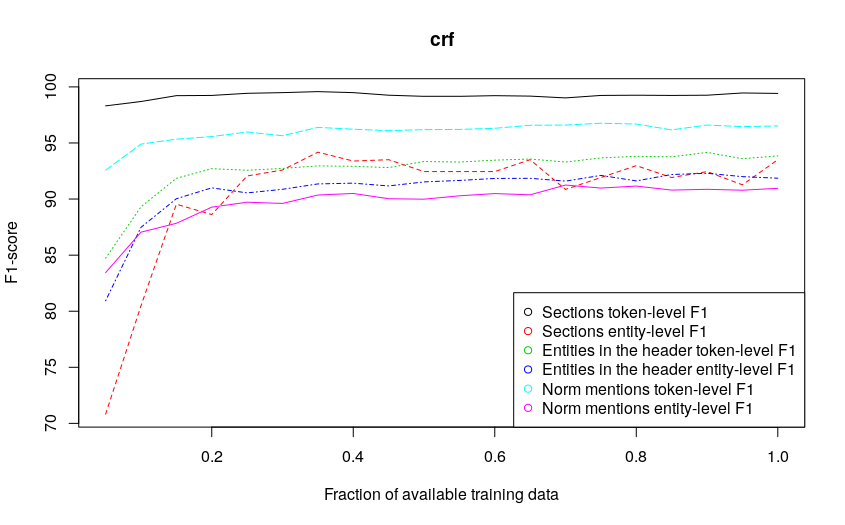
\includegraphics[width=0.9\textwidth]{lc-crf.png}
\caption{Résultats en fonction du nombre de données d'entrainement (fractions d'environ 380 décisions)}\label{p4_crf-learning-curves}
\end{figure}
\end{frame}

\section{Extraction d'informations sur les demandes}

\begin{frame}{Extraction des informations sur les demandes}
\begin{block}{Informations pertinentes à extraire}
\begin{itemize}
\item \textbf{Position de la partie}: Intimé
\item \textbf{Catégorie de demande}: Dommages-intérêts pour procédure abusive
\begin{itemize}
\item \textbf{Objet}: Dommages-intérêts
\item \textbf{Fondement}: Articles 1382 code civil et 32-1 code de procédure civile
\end{itemize}
\item \textbf{Quantum demandé}: 20 000 euros
\item \textbf{Résultat} : Rejet
\item \textbf{Quantum accordé} : 0 euros
\end{itemize}
\end{block}
\end{frame}

\begin{frame}{Difficultés}
%\small
Expressions non structurées, par  \textcolor{orange}{référence}, par \textcolor{blue}{agrégation}

\begin{exampleblock}{Expression de demande}
La société A. conclut à la confirmation du jugement entrepris sauf à
former appel incident sur la disposition du jugement l'ayant déboutée de sa
demande de \textbf{dommages intérêts pour abus de procédure} et elle demande à la cour de
condamner l'appelante à lui payer la somme de \textbf{20 000 euros} à titre de dommages
intérêts ...

%CATOU972015.xml
%Aux termes de ses conclusions ..., la S.A.S. S. présente \textcolor{orange}{les mêmes demandes que celles de la S.A. V. F.}

%- \textbf{la} condamner à payer une somme de \textbf{283 589 euros} à titre de {\bf dommages et intérêts pour concurrence déloyale},

\end{exampleblock}

\begin{exampleblock}{Expression de resultat}
La cour, ... 

Confirme \textcolor{orange}{la décision entreprise} en \textcolor{blue}{toutes ses dispositions},
\end{exampleblock}
\end{frame}

\begin{frame}{Approche supervisée d'extraction des demandes}
\begin{block}{Simplification du problème}
\begin{itemize}
\item On suppose qu'une décision ne comprend qu'au plus une demande d'une catégorie donnée
\item Méthode générique qui s'adapte aux spécificités de la catégorie traitée
\item Définition incrémentale des catégories
\end{itemize}
\end{block}
\end{frame}

%\begin{frame}{Détection d'une catégorie par classification}
%\begin{figure}
%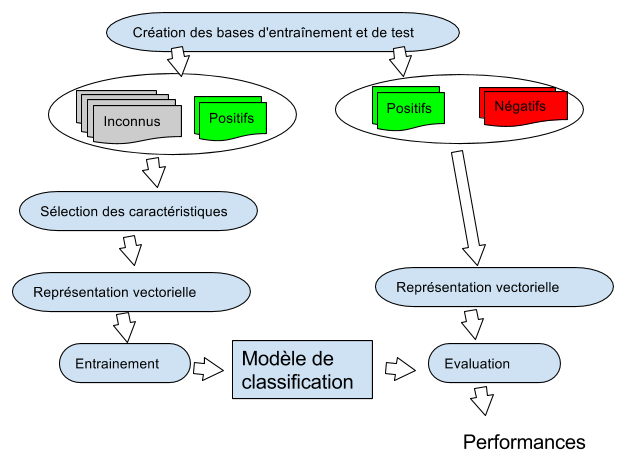
\includegraphics[scale=0.6]{archi-classif.png}
%\caption{Approche d'expérimentation de la classification}
%\end{figure}
%\end{frame}

\begin{frame}{Approche supervisée d'extraction des demandes}
(1) Sélection de termes caractéristiques
\begin{exampleblock}{Dommages-interets pour abus de procedure}
\small
\begin{tabular}{l|c}
\textbf{Terme (n-gram)} & \textbf{Poids global (NGL)}  \\ \hline
\midrule
procédure abusive & 15.710 \\ \hline
pour procédure abusive & 15.007 \\ \hline
pour procédure & 14.890 \\ \hline
abusive & 13.721 \\ \hline
intérêts pour procédure & 10.306 \\ \hline
abus & 10.288 \\ \hline
intérêts pour procédure abusive & 9.984 \\ \hline
32-1 & 9.534\\ \hline
%et intérêts pour procédure & 9.341 \\ \hline
%dommages et intérêts pour procédure & 9.341 \\ \hline
... & ...
\end{tabular}
\end{exampleblock}
$ngl(w,c) = \frac{\sqrt{N} ((N_{w,c} N_{\overline{w},\overline{c}}) - (N_{w,\overline{c}} N_{\overline{w},c}))}{\sqrt{N_w N_{\overline{w}} N_c N_{\overline{c}}}}$ \cite{ng1997ngl}
\end{frame}

%\begin{frame}{Catégorisation semi-supervisée des décisions}
%\begin{figure}
%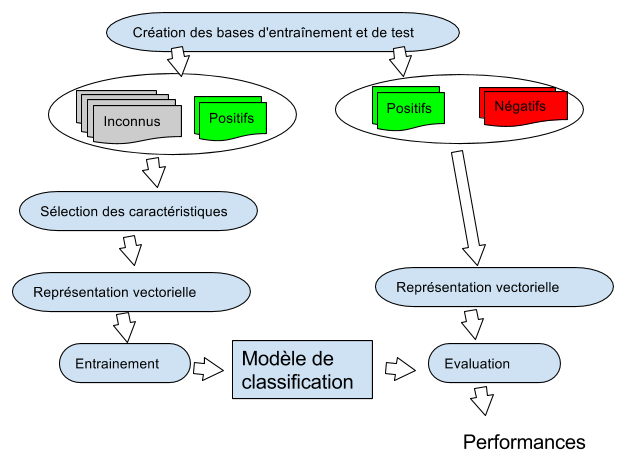
\includegraphics[scale=0.6]{archi-classif.png}
%\caption{Approche d'expérimentation de la classification}
%\end{figure}
%\end{frame}

\begin{frame}{ Détection d'une catégorie par classification binaire}

Conditions d'expérimentation

\begin{itemize}
\small
\item Représentation vectorielle: {\small \[ poids(w*, t) = poids_{local}(w*, t) * poids_{global}(w*) * facteur_{normalisation}\]}
\item Évaluation de différentes configurations:
\begin{itemize}
\item dimensions des vecteurs : 10, ..., 250, ...
\item méthodes de sélection de termes discriminants: $\chi^2, \Delta_{DF}, Marascuilo, NGL, GSS $  ...
\item méthodes de classification: SVM, arbre de décision, KNN, naïf bayésien (avec Weka\cite{Eibe2016Weka})
\item méthodes de pondération locale : TF, LogTF, ATF, TP
\end{itemize}
\item environ 2000 cas inconnus, 
\item dommages-intérêts pour abus de procédure : entrainement 152 positifs, test 39 positifs + 157 négatifs
\item prestation compensatoire : entrainement 100 positifs, test 100 positifs + 100 négatifs
\end{itemize}
\end{frame}

\begin{frame}{Détection d'une catégorie par classification binaire}

Premiers résultats:

%{\small $ poids(w*, t) = poids_{local}(w*, t) * poids_{global}(w*) * facteur_{normalisation}$}

\begin{figure}
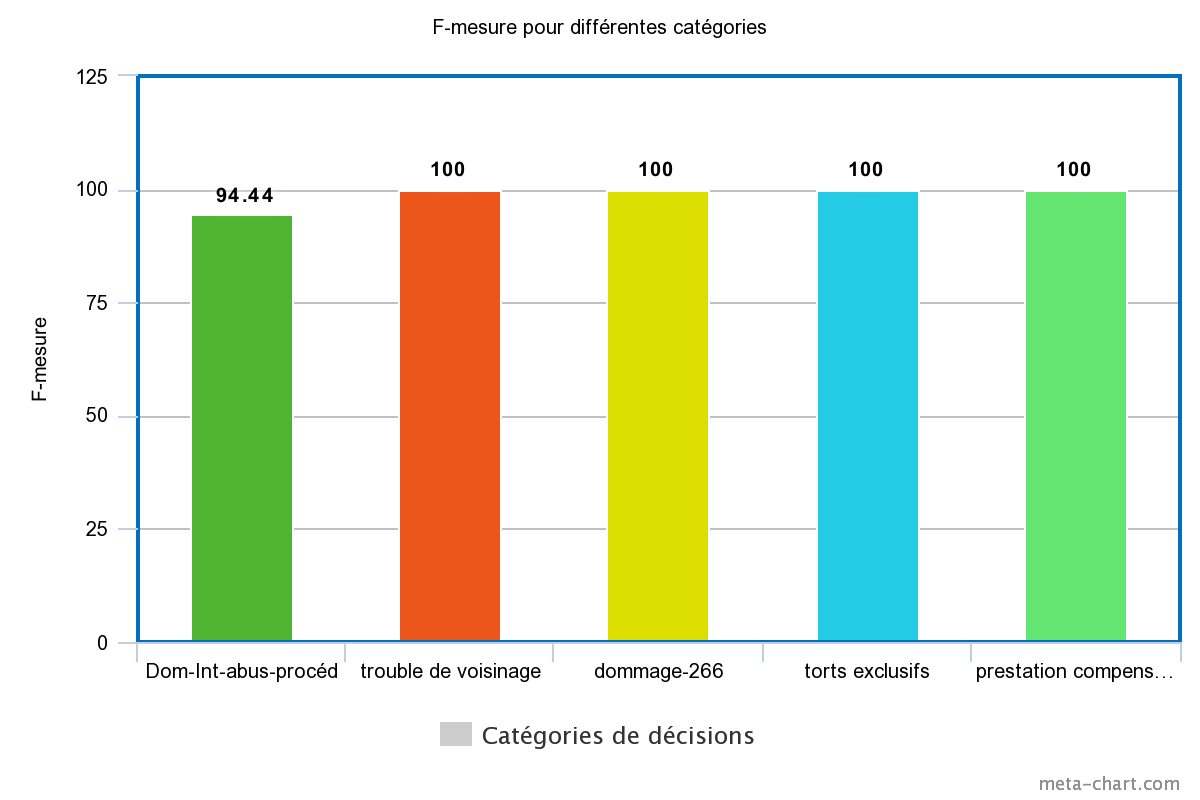
\includegraphics[width=0.75\textwidth]{f-mesure-classif.png}
\caption{Résultats des meilleures configurations (taille des vecteurs, poids global, poids local, modèle de classifieur)}
\end{figure}
\end{frame}

\begin{frame}{Extraction du sens du résultat (avec la même approche)}
Classification des décisions d'une catégorie prédéfinie
\begin{figure}
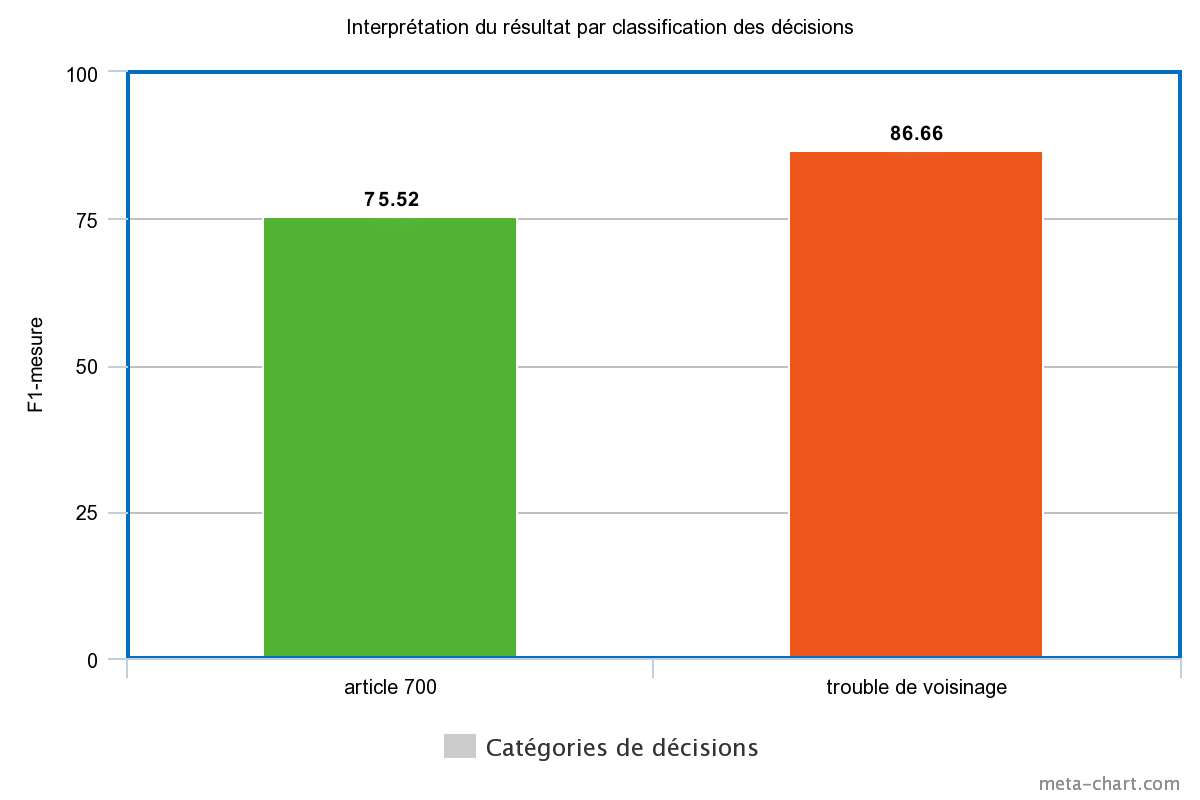
\includegraphics[width=0.8\textwidth]{classifResultat.png}
\caption{Résultats des meilleures configurations (taille des vecteurs, poids global, poids local, modèle de classifieur)}
\end{figure}
\end{frame}

\begin{frame}{Extraction du sens du résultat (méthodes Gini-PLS)}

Combinaison de 2 méthodes de régression:
\begin{enumerate}
\setlength\itemsep{1.5em}
\item PLS: réduction supervisée des dimensions $x_1, x_2, ..., x_p$ en composantes orthogonales $t_1, ...., t_h$

$t_h = w_{h1} x_1 + \cdots + w_{hj} x_j + \cdots + w_{hp} x_p$

avec $w_{hj} = \frac{cov(u_{(h-1)j}, \epsilon_h)}{\sqrt{\sum_p^{j=1} cov^2(u_{(h-1)j}, \epsilon_h)}}$
, $y=c_1 t_1 + ... + c_h t_h + \epsilon_h$,

et $x_j=\beta_{1j} t_1 + ... + \beta_{hj} t_h + u_{(h-1)j}$

\item Gini: élimination de la sensibilité au \textit{outliers} en remplaçant la covariance $cov(x_j, y)$ par la covariance de Gini $cog(y; x_j) := cov(y; R(x_j))$
\end{enumerate}

\cite{souissi2013gini}

\end{frame}

\section{Activités complémentaires}
\begin{frame}{\currentname}
\begin{itemize}
\setlength\itemsep{1em}
\item Formations complémentaires: 11 modules (132h)
\item Enseignement: travaux pratiques (Big Data avec Hadoop)
\item Valorisation des travaux: 
\begin{itemize}
\item Conférence EGC, Grenoble, janvier 2017
\item 1 article en relecture (AKDM8)
\item Démo des 1er résultats: SAT AXLR (Montpellier)
\item Séminaire e-juris (Lyon)
\end{itemize}
\item Participation au challenge COLIEE: 4e place / 12
\end{itemize}
\end{frame}

\section{Conclusion et plan de travail}

\begin{frame}{Résumé}
\begin{itemize}
\item Détection d'entités et de sections basée HMM / CRF
\begin{itemize}
\item Bons résultats même avec un peu de données annotées
\item Difficultés:
\begin{itemize}
\item Annotation manuelle d'un jeu suffisant d'exemples
\item Identification de bons descripteurs 
\item Lenteur de la sélection de caractéristiques
\end{itemize}
\item Limite de l'approche:
\begin{itemize}
\item Descripteurs définis manuellement 
\item Etiquetage en plusieurs passes 
\end{itemize}
\end{itemize}
\item Détection de termes propres aux catégories de demandes
\item Détection des catégories par classification
\item Détection moins triviale du sens du résultat 
\end{itemize}

\end{frame}

\begin{frame}{Organisation du travail en 3 problématiques}

\begin{enumerate}
\setlength\itemsep{1.5em}
\item Extraction des demandes et résultats par affinement de la segmentation des textes
%\item Catégorisation supervisée vs. non-supervisée des demandes extraites 
\item Standardisation et représentation des informations extraites sous forme de base de connaissances
\item Détermination des facteurs associables aux décisions des juges (faits ou arguments)

\end{enumerate}

\end{frame}

\section{Questions?}

%\begin{frame}{Quelle aide à l' \og analyse \fg{} est précisément attendue?}
%\begin{enumerate}
%\setlength\itemsep{2em}
%\item Comparaison des taux des types de résultat : 
%
%positif vs. négatif ...
%\begin{itemize}
%\setlength\itemsep{1em}
%\item pour une catégorie définie de demandes
%\item dans une situation factuelle d'intérêt
%\end{itemize}
%\item Détermination d'idées associées à un type de résultat 
%\begin{itemize}
%\setlength\itemsep{1em}
%\item faits
%\item arguments
%\end{itemize}
%\end{enumerate}
%\end{frame}
%
%\begin{frame}{Organisation prévisionnelle de la rédaction}
%\begin{enumerate}
%\item Introduction (Positionnement, Attendu, défis, généralités sur les compétences techniques nécessaires)
%\item Étude bibliographique: Analyse sémantique et prédictive des décisions judiciaires
%\item Extraction/détection d'information à partir de texte: expression et résolution d'entités, de demandes et de résultats, liaison des demandes et résultats correspondances
%\item Interprétation: Catégorisation des demandes et résultats
%\item Explication : détermination des facteurs liés au sens du résultat
%\item Conclusion: apport, voies d'amélioration, autres problématiques  
%\end{enumerate}
%\end{frame}

%-=-=-=-=-=-=-=-=-=-=-=-=-=-=-=-=-=-=-=-=-=-=-=-=
%	References:
%-=-=-=-=-=-=-=-=-=-=-=-=-=-=-=-=-=-=-=-=-=-=-=-=
\begin{frame}[t,allowframebreaks]{References}
\tiny
\bibliographystyle{apalike}
\bibliography{references}	
\end{frame}

\end{document}
